%%%%%%%%%%%%%%%%%%%%%%%%%%%%%%%%%%%%%%%%%
% Thin Sectioned Essay
% LaTeX Template
% Version 1.0 (3/8/11)
%
% This template has been downloaded from:
% http://www.LaTeXTemplates.com
%
% Original Author:
% Nicolas Diaz (nsdiaz@uc.cl) with extensive modifications by:
% Vel (vel@latextemplates.com)
%
% License:
% CC BY-NC-SA 3.0 (http://creativecommons.org/licenses/by-nc-sa/3.0/)
%
%%%%%%%%%%%%%%%%%%%%%%%%%%%%%%%%%%%%%%%%%

%----------------------------------------------------------------------------------------
%	PACKAGES AND OTHER DOCUMENT CONFIGURATIONS
%----------------------------------------------------------------------------------------

\documentclass[a4paper, 11pt]{article} % Font size (can be 10pt, 11pt or 12pt) and paper size (remove a4paper for US letter paper)

\usepackage[protrusion=true,expansion=true]{microtype} % Better typography
\usepackage{graphicx} % Required for including pictures
\usepackage{wrapfig} % Allows in-line images

\usepackage{mathpazo} % Use the Palatino font
\usepackage[T1]{fontenc} % Required for accented characters
\linespread{1.05} % Change line spacing here, Palatino benefits from a slight increase by default

\makeatletter
\renewcommand\@biblabel[1]{\textbf{#1.}} % Change the square brackets for each bibliography item from '[1]' to '1.'
\renewcommand{\@listI}{\itemsep=0pt} % Reduce the space between items in the itemize and enumerate environments and the bibliography

\renewcommand{\maketitle}{ % Customize the title - do not edit title and author name here, see the TITLE block below
\begin{flushleft} % Right align
{\LARGE\@title} % Increase the font size of the title

\vspace{50pt} % Some vertical space between the title and author name

{\large\@author} % Author name
\\\@date % Date

\vspace{40pt} % Some vertical space between the author block and abstract
\end{flushleft}
}

%----------------------------------------------------------------------------------------
%	TITLE
%----------------------------------------------------------------------------------------

\title{\textbf{NIKA2 research note}\\   
\textsc{NIKA2 Commissioning results v1.0}} % Subtitle


\author{NIKA2 team % Author
\\{\textit{NIKA2 collaboration}}} % Institution

\date{\today} % Date



%----------------------------------------------------------------------------------------

\begin{document}

\maketitle % Print the title section
\tableofcontents
%----------------------------------------------------------------------------------------
%	ABSTRACT AND KEYWORDS
%----------------------------------------------------------------------------------------

%\renewcommand{\abstractname}{Summary} % Uncomment to change the name of the abstract to something else

\begin{abstract}
This notes describe the main results of the NIKA2 commissioning campaigns.
\end{abstract}

%\hspace*{3,6mm}\textit{Version:}  % Version

\vspace{30pt} % Some vertical space between the abstract and first section

%----------------------------------------------------------------------------------------
%	ESSAY BODY
%----------------------------------------------------------------------------------------

%\tableofcontents

\section{Introduction}

\subsection{Commissioning goals}
The main goal of the NIKA2 commissioning runs described below is to check the performance of the instrument and its stability with respect to the specifications described in Table \ref{nika2specs}.

%\begin{table}[h]
%\caption{Commissioning campaigns and dates}
%\label{nika2specs}
%\begin{tabular}{|c|c|c|s}
%\hline 
% FWHM &   &  \\
%\hline  
%\hline 
%\end{tabular} 
%\end{table} 



\subsection{Commissioning runs}
We had 9 commissioning runs for NIKA2 as described in Table~\ref{nika2runs}.

%\begin{table}[h]
%\caption{Commissioning campaigns, dates and general comment%
%\label{nika2runs}
%\begin{tabular}{|c|c|c|}
%\hline 
%RUN  &  Dates & General comments \\ 
%\hline 
%N2R1 &      xx  &  xx \\  
 
%\hline 
%\end{tabular} 
%\end{table} 

% ---------------------------------------
\section{Bandpasses}
\begin{figure}[ht] % Inline image example
\begin{center}
\includegraphics[width=0.9\textwidth]{Figures/SpectralBands/atm_transmission.pdf}
\caption{Spectral transmission of the the three NIKA2 arrays as a function of frequency in GHz. For illustration we also plot the ATM atmospheric model for different values of pwv. \label{spectralband}}
\end{center}
\end{figure}


\begin{figure}[ht] % Inline image example
\begin{center}
\includegraphics[width=\textwidth]{Figures/SpectralBands/opacity_ratio_vs_tau1.pdf}
\caption{Expected atmospheric opacity ratio of the 2 and 1 mm channels as function of the opacity at 1 mm. \label{thopacities}}
\end{center}
\end{figure}



The NIKA2 spectral bands were measured in the laboratory using a Martin Pupplet interferometer.
Both arrays and filter bands were considered in the measurements. Theser were obtained from the difference of two black-bodies, hence they include a a $\nu^2$ RJ term. During the commissioning in Run 5 array 2 was replaced. The new array has a different spectral transmission. Figure shows the spectral transmissions for the three arrays. Notice that array A2 was replaced by a new on in N2R5 and that the spectral transmissions are not the same (red and cyan lines in the figure).


\begin{table}[h]
\caption{Spectral transmission characteristics for the NIKA2 arrays.%
\label{nika2runs}}
\begin{tabular}{|c|c|c|c|c|}
\hline 
  &     A1  &  A3 &  A2 2015 & A2 2016 \\ 
\hline 
Central Frequency [GHz] &   255.5  & 257.8   &   147.7  & 151.6 \\  
Bandwidth [GHz]         &   47.8   & 45,7    &   41.8   & 42.1 \\
\hline 
\end{tabular} 
\end{table} 


%What actually matters more than the ``central frequency'' that depends on many
%assumptions and definitions are the bandpasses. We should make available in a
%.fits file, clearly, our bandpasses to avoid future misunderstanding and propagation of
%false numbers. Official values should be 150 and 260~GHz. We should also clearly
%state that these measured bandpasses were done with the difference of two
%black-bodies, hence they include a $\nu^2$ RJ term.\\

Using the NIKA2 bandpasses for N2R9, we can integrate the ATM atmospheric model to compute the expected ration between the atmospheric opacity for the two NIKA2 channels. This shown in Figure~\ref{thopacities} where we present the atmospheric opacity ratio of the 2 and 1 mm channels as a function of the opacity for the 1 mm one.



% ---------------------------------------
\section{sensitivities}

\begin{figure}
\begin{center}
%\includegraphics[clip, angle=0, scale =
%  0.5]{Figures/NEFD_HLS091828_20170226s415_FXDC0C1_GaussPhot.png}
\includegraphics[clip, angle=0, scale = 0.5]{Figures/nefd_mpfit_HLS091828.eps}
\caption{Kids Xcalib with fixed fwhm 12.5 and 18.5, HLS091828.}
\label{fig:nefd_vs_t}
\end{center}
\end{figure}

{\bf The specs/goals ``NEFD on X \% of pixels'' should be understood as : we have
XX\% valid pixels, and with these pixels, we have an NEFD of YY. We should not
discard some fraction of our pixels and estimate an NEFD on this subset.}\\

HLS091828 is moderately faint source, expected to be below 100~mJy at 1mm and
XX~mJy at 2mm {\bf check values in NIKA1 paper + use SED for predictions in
  NIKA2's bands}. This source was chosen for its flux and its availability during
Run9 for long integration. It has been observed for XX hours in total over three
nights.

\subsection{Data processing}

The data were decorrelated using the XXX method... The scans have been combined
with standard inverse noise weighting. The noise in each map pixel is derived
from the rms of the background corrected for the number of observations per
pixel.

\subsection{NEFD Methods 1 and 2: deep integration}
These data can be used to derive the NEFD in several ways. One is to fit the
evolution of the uncertainty on the flux of the source $\sigma_\phi$ with the
integration time. Another one is to produce jackknife maps with the data and to
measure the uncertainty on the flux in the end, while estimating the time of
integration. Results are summarized in Tab.~\ref{tab:nefd}.

Fig.~\ref{fig:nefd_vs_t} shows the decrease of the uncertainty on the measured
flux at the center of the map as a function of time. We either fit a power law
or fix the power law to -0.5 and fit only the amplitude. Uncertainties on these
values have been estimated via a bootstrap method: we randomize the scans and
derive the standard deviation of the average of $n$ scans for any $n$ between 1
and the total number of scans. This gives us an estimate of the uncertainty on
$\sigma_\phi$ for a time of integration corresponding to $n$ scans. Strictly
speaking, all the scans do not have the exact same duration, but the difference
is negligible here.


\begin{table}
\begin{tabular}{|l|l|l|l|l|}
\hline
Array & Free power law & Fixed power law $t^{-0.5}$ & Jackknife & Tau and air mass\\
\hline
A1       & $47.9$ mJy.s$^{-0.54}$ & $37.9$ mJy.s$^{1/2}$ & 35.6 mJy.s$^{1/2}$ & {\bf TBD}\\
A2       & $5.2$  mJy.s$^{-0.51}$ & $4.8$  mJy.s$^{1/2}$ & 5.7  mJy.s$^{1/2}$ & {\bf TBD}\\
A3       & $38.9$ mJy.s$^{-0.54}$ & $30.6$ mJy.s$^{1/2}$ & 30.4 mJy.s$^{1/2}$ & {\bf TBD}\\
A1 \& A3 & $28.5$ mJy.s$^{-0.53}$ & $23.6$ mJy.s$^{1/2}$ & 22.4 mJy.s$^{1/2}$ & {\bf TBD}\\
\hline
\end{tabular}
\label{tab:nefd}
\end{table}


\begin{figure}
\begin{center}
\includegraphics[clip, angle=0, scale =0.8]{Figures/NEFDIndScans/nefd_tau_run22.pdf}
\caption{Astronomer NEFD as a function of atmospheric background for the 1 (orange dots) and 2 (cyan dots) mm channels. We also show the expected NEFD evolution with atmospheric background (red and blue curves)}
\label{fig:nefdvsbackground}
\end{center}
\end{figure}

\subsection{NEFD Method 3: scan NEFD vs opacity and air mass}
\begin{figure}
\begin{center}
\includegraphics[clip, angle=0, scale =0.8]{Figures/NEFDIndScans/nefd_evol_run22.pdf}
\caption{Evolution of the measured instrument NEFD across scans for N2R9.}
\label{fig:nefdvsscans}
\end{center}
\end{figure}

\begin{figure}
\begin{center}
\includegraphics[clip, angle=0, scale =0.8]{Figures/NEFDIndScans/nefd_flux1mm_run22.pdf}
\caption{Measured instrument NEFD as a function of the flux of the source.}
\label{fig:nefdvsflux}
\end{center}
\end{figure}
\begin{figure}
\begin{center}
\includegraphics[clip, angle=0, scale =0.8]{Figures/NEFDIndScans/hist_nefd_ref_run22.pdf}
\caption{Histogram of the measured reference NEFD across the N2R9 for the 1 (right) and 2 (left) mm channels.}
\label{fig:nefdhist}
\end{center}
\end{figure}
 

In this section we investigate the astronomer NEFD as a function of the atmospheric opacity and air mass. Figure~\ref{fig:nefdvsbackground} shows the measured NEFD, which we refer to as astronomer NEFD, for the 1 and 2 mm as a function of the measured atmospheric background in terms of $\tau/sin(El)$. The atmospheric opacity was computed as discussed in Section~\ref{se:opacities}. We observe that the increase of the astronomer NEFD is in agreement with what we would expect for background dominated sensitivity. We observe however some significant deviations from the curve. To investigate this issue we also show in Figure~\ref{fig:nefdvsscans} the evolution of the background corrected NEFD, hereafter instrument NEFD, across the N2R9 campaign for arrays A1 (blue), A3 (green) and A2 (cyan), and for the combination of A1 and A3 (red). We globally obseve stable NEFD across the run, with A1 sensitivity being worse than for A3. We also show the measured instrument NEFD as a function of the flux of the source in the 1 mm channel in Figure~\ref{fig:nefdvsflux}. We observe that the observed deviations in the instrument NEFD correspond mainly to the large flux source scans. This is more obvious in Figure~\ref{fig:nefdhist} where we present the histogram of the measured NEFD for 2 mm of pwv and at a elevation of 60 degrees, hereafter, reference NEFD, for the 1 and 2 mm channels.



% ---------------------------------------
\section{Focal plane reconstruction}
\label{se:fov}

\begin{figure}
\begin{center}
\includegraphics[clip, angle=0, scale = 0.15]{Figures/FOV_A1.png}
\includegraphics[clip, angle=0, scale = 0.15]{Figures/FOV_A2.png}
\includegraphics[clip, angle=0, scale = 0.15]{Figures/FOV_A3.png}
\caption{Nasmyth offsets of each array, from beammap 26s415 on 3C84.}
\label{fig:fov}
\end{center}
\end{figure}

\begin{table}
\begin{tabular}{|l|l|l|}
\hline
Array & Number of valid kids & Fraction of all kids\\
\hline
A1 & 793 & 0.75\\
A2 & 481 & 0.83\\
A3 & 872 & 0.83\\
\hline
\end{tabular}
\end{table}

\begin{equation}
FOV diameter = \sqrt{4 N_{tot. kids} * gridstep^2/\pi}
\end{equation}

The same definition applies to ``Effective FOV'' to avoid extra multiplication
by the fraction of valid pixels

\begin{equation}
F\lambda = gridstep\times D(30m)/\lambda
\end{equation}

% ----------------------------------------
\section{Opacity derivation}
\label{se:opacities}

For each kid $k$, $f_{tone}^k$ moves with the atmospheric load according to

\begin{equation}
f_{tone}^k = C_0^k + C_1^k T_{atm}[1-e^{-\tau/\sin\delta}]
\end{equation}

where $\delta$ is the elevation. The {\tt skydip} procedure consists in moving
the telescope in elevation step by step and to monitor, for each kid, the
evolution of $f_{tone}^k$ vs the air mass and to fit the opacity $\tau$ and
$C_0^k$ and $C_1^k$. All the skydips (that were obtained under various opacity
conditions) are analysed together to break the degeneracies between these
parameters. The procedure has two steps. First, all the skydips are analysed
individually to simply measure $f_{tone}^k$ for each stable elevation and fit
simultaneously all the parameters. Error bars on $\tau$ are estimated by doing
this procedure on blocks of 40 kids only and getting a dispersion on the
resulting $\tau$ from the different blocks. Usually the dispersion comes out as
$4\times 10^{-3}$ at 1mm and $1\times 10^{-3}$ at 2mm. Once the $\tau$ values
are estimated for each skydip (as the average over the blocks), we compute
(while fixing $\tau$) the $C_0$ and $C_1$ final values for each kid. We thus
retrieve the coefficients of all the Kids even though some of them could not
contribute to the tau determination.

%% \begin{figure}
%% \begin{center}
%% \includegraphics[clip, angle=0, scale =
%%   0.5]{Figures/NEFD_vs_tau_20170226s415_FXDC0C1_Jy_common_mode_kids_out.png}
%% \includegraphics[clip, angle=0, scale =
%%   0.5]{Figures/tau1_tau2_20170226s415_FXDC0C1_GaussPhot_common_mode_kids_out.png}
%% \caption{}
%% \label{fig:fov}
%% \end{center}
%% \end{figure}

\begin{figure}
\begin{center}
\includegraphics[clip, angle=0, scale = 0.5]{Figures/test_allskd_N2R9.jpg}
\caption{{\bf Fix me : improve plot quality and plot only the 3rd one.}}
\label{fig:test_allskd_N2R9}
\end{center}
\end{figure}

%------------------------------------------
\section{Beam pattern}
%%
%%
%%      SECTION: BEAM PATTERN 
%%

%% [intro]
%%________________________________________________________

The NIKA2 beam pattern mainly depends on the IRAM 30m telescope and
NIKA2 full (external and internal) optical system characteristics,
whereas the detectors themselve might have an impact at sub-dominant
level (through e.g. time constants or correlated noises). In this
section, first we reconstruct the focus surfaces and present the
optimal focus, then we characterize both the main beam, which is
modeled as an elliptical Gaussian, and the full beam pattern including
error beams up to angular scales of 10 arcmin.



%% [Optimal Focus]
%%________________________________________________________
\subsection{Optimal focus}
\label{sec:focus}

Owing to the NIKA2 $6.5~\rm{arcmin}$ FOV, the focus is expected to
slightly changes across the FOV, defining curved focal surfaces at the
location of the three arrays. Therefore, beam patterns are expected to
show some scatter across the FOV accordingly to the focal
surfaces. Although all the detectors cannot be individually focalised,
an optimal axial focus of the telescope can be found to maximize the
number of detectors at the best focus and hence, maximize the
resolution of the NIKA2 maps. This optimal z-focus setting is obtained
in measuring the focus at the center of the arrays as described
Sect.~\ref{sec:focus-meas} and apply a focus shift, which is primary
predicted using Zemax simulation, and ultimately verified by measuring
the focus surfaces, as decribed in Sect.~\ref{sec:focus-surf}.


\subsubsection{Focus estimation}
\label{sec:focus-meas}

The best axial focus in the central region of the arrays is estimated
using the so-called 'focus$\_$OTF' PAKO script, which realises a
series of five $1' \times 5'$ OTF scans at various values of
the focus in $0.4~\rm{mm}$-steps around an \emph{a priori} value $z_0$,
namely $z \in \{-0.8, -0.4, 0, 0.4, 0.8\} + z_0$. Elliptical Gaussian
fits on the reconstructed maps provide estimates of the flux and FWHM
along minor- and major-axis for each focus. Then, parabolic fits are
used to determine the best focus. We consider three estimates: i)
$\hat z_{\rm{peak}}$ the focus that maximizes the estimated flux,
which is the amplitude of the 2D Gaussian, 
ii) $\hat z_{\rm{fwhm}}$ the focus that
minimizes the geometrical FWHM, defined as the quadratic mean of
$\rm{FWHM}_{\rm{major}}$ and $\rm{FWHM}_{\rm{minor}}$,  and iii)
$\hat z_{\rm{ellipt}}$ the focus that minimizes the beam ellipticity,
defined as $\rm{FWHM}_{\rm{major}}/\rm{FWHM}_{\rm{minor}}$.
Fig.~\ref{fig:focus-example} shows an example of
axial focus measurement using a 'focus$\_$OTF' observation of Neptune
during N2R10.

\begin{figure}
\begin{center}
  \includegraphics[clip, angle=0, scale=0.25]{Figures/plot_20170419s143.png}
\caption{Example of axial focus measurment using a 'focus$\_$OTF' observation of Neptune
during N2R10 [PLACEHOLDER]}
\label{fig:focus-example}
\end{center}
\end{figure}


\subsubsection{Focus consistency between arrays}

{\bf refaire les plots de difference de focus entre matrices }

\subsubsection{Reconstruction of the focus surfaces}
\label{sec:focus-surf}

\begin{figure}
\begin{center}
  \includegraphics[trim={0, 1cm, 0, 1cm}, clip, angle=0, scale=0.5]{Figures/fov_focus_mv_5.png}
\caption{Focus surface of A1, A3 and A2 arrays from left to
  right. From top to bottom, the focus estimates rely on
  FWHM-minimization, amplitude-maximization of an elliptical
  Gaussian of fixed FWHMs and amplitude-maximization of an elliptical
  Gaussian.}
\label{fig:focus-surfaces}
\end{center}
\end{figure}

\emph{Method. } We measure NIKA2 focal surfaces by means of a sequence of five 'beam-map'
scan observations of bright point-like sources, typically Planets or
bright quasars,
for various settings of the telescope axial focus around the
optimal focus $z_{\rm{opt}}$. A beam-map scan consists of a deep-integrated
$13.5' \times 7.8'$ OTF-scan observation comprizing $99$ sub-scans and
with a scanning speed of either $65''/s$ whenever the mean integration
elevation is $< 60$ degree or $39"/s$ at higher elevation. The z-focus is changed in step of
$0.6~\rm{mm}$ to probe a large focus range for measuring even the
extreme variation of the focus surfaces,
namely $z \in \{-1.2, -0.6, 0, 0.6, 1.2 \} + z_{\rm{opt}}$.
Each beam-map scans allow for $4''$-resolution individual maps per kid to
be projected. Before the projection, the correlated noise is mitigated
from each KID timeline in subtrating out a common mode, which is obtained
using, amongst the other detectors, those that correlates the most
with this KID and that are located outside a radius of $90''$
around the source centroid.
Therefore, a series of five cleaned maps at various focus is
available for each detector, from which the best focus is estimated as
described in Sect.~\ref{sec:focus-meas}. The ensemble of the relative
focus estimate per KIDs with respect to the best focus at the center
of the array constitutes the focus surface. An accurate estimate of
the center focus is obtained as the
weighted average focus estimate of the KIDs lying in a $30''$ radius
around the geometrical center of the array. This average does not
induce any sizeable bias thanks to the flatness of the focus surface
in the innermost regions. For robustness test, we consider three focus
estimates: the two first ones are the same as discussed in
Sect.~\ref{sec:focus-meas} -- namely i) $\hat z_{\rm{fwhm}}$ the focus that
minimizes the geometrical FWHM and ii) $\hat z_{\rm{peak}}$ the focus
that maximizes the amplitude of the best-fitting ellitical Gaussian --
whereas the third one is $\hat z_{\rm{flux}}$ the focus that maximizes
the amplitude of the best-fitting elliptical Gaussian of fixed FWHM
(at $12''$ at $260~\rm{GHz}$ and $18''$ at $150~\rm{GHz}$). The 
comparison between the two amplitude-based estimators
($\hat z_{\rm{peak}}$ and $\hat z_{\rm{flux}}$), will test the
stability of the focus results against the exact choice of the beam fitting
function. Since the ellipticity-based estimator $\hat z_{\rm{ellip}}$ is
less sensitive to focus changes and yields larger uncertainties than the
others, we do not use it for the focus surface reconstruction.     


\emph{Data selection. }
During the three commissioning campaigns that occured after the change of A1
lens and the improvement of internal optics alignment (hence in the
final NIKA2 optic configuration),
nine out-of-focus
beam-map scan sequences have been acquired, including incomplete
sequences and sequences hindered by poor atmospheric conditions. We
select sequences that i) comprises at least four scans, ii) have been
observed at zenith opacity at $225~\rm{GHz}$ (as indicated by
the IRAM taumeter) below 0.5 and iii) have a maximal central focus
drift between the starting time and the end of the sequence of
$0.5~\rm{mm}$. These criteria preserve five sequences from which focus
surfaces can be reconstructed. Namely, we consider the sequences
$20170226s415\mbox{--}419$, $20170419s133\mbox{--}137$, $20170420s113\mbox{--}117$,
$20170421s160\mbox{--}164$ and $20170424s123\mbox{--}127$, which consist of observations
of the bright quasar '3C84' and Neptune.

\emph{Results. }
For each detector $k$ and each beam-map sequence $s$, we obtain for
the array $a$, a focus measurement $z_k^{a, s} \pm \sigma_k^{a, s}$,
where $\sigma_k^{a, s}$ is the $1\mbox{--}\sigma$ error of the least-square
polynomial fit. The focus surface measurements per array obtained from the five
beam-map sequences are combined using an inverse-variance weighting
scheme to obtain the focus surface estimates 
\begin{equation}
\label{eq:mv_focus_surf}
z_k^{(a)} = \left( \sigma_k^{(a)} \right)^2 \,  \sum_s \frac{z_k^{a,s}}{\left(\sigma_k^{a,s}\right)^2}\, \,  ,
\end{equation}
with uncertainties 
\begin{equation}
\label{eq:error_mv_focus_surf}
\sigma_k^{(a)} = \left[ \sum_s \frac{1}{\left(\sigma_k^{a,s}\right)^2}\right]^{-1/2}\, .
\end{equation}


We present NIKA2 focus surfaces per arrays obtained as in
Eq.~\ref{eq:mv_focus_surf} 
%from the inverse-variance weighted combination of the five
%reconstructed focus surfaces per arrays
in Fig.~\ref{fig:focus-surfaces}.
The three flavours of focus-estimators provide us with focus surfaces
per arrays that are in good agreement with each others and that have a
non-axisymetrical flatten bowl shape consistent with expectations from
simulation {\bf [TBA, as discussed further below]}.
The median defocus (that is the relative focus w.r.t. the center)
across the detectors is about
$-0.1~\rm{mm}$ for the three arrays. Maximal defocus values of about
$-0.6~\rm{mm}$ are found for detectors located in the outer top and
left regions of the FOV. Finally, a fraction comprised between $20$
and $30\%$ of the KIDs has a relative $z\le -0.2~\rm{mm}$.  

We primarily estimate the uncertainty of the focus
surface measurements using the standard deviation between the three
estimators $z_k^{(a)}|_{\rm{fwhm}}$, $z_k^{(a)}|_{\rm{peak}}$ and
$z_k^{(a)}|_{\rm{flux}}$. We found approximatively homogeneous
standard deviation surfaces per arrays, which have median values across
the FOV of about $0.03~\rm{mm}$.
However, we cross-check this error estimate by forming the quadratic mean of
the three inverse-variance error surfaces per arrays, which are defined in
Eq.~\ref{eq:error_mv_focus_surf} and quoted
$\sigma_k^{(a)}|_{\rm{fwhm}}$, $\sigma_k^{(a)}|_{\rm{peak}}$ and
$\sigma_k^{(a)}|_{\rm{flux}}$. This provides us with more optimistic
error surfaces per array, which do not show any clear pattern across
the FOV and which have a median value across the detectors of about
$0.015~\rm{mm}$.  

%[EXPAND THE DISCUSSION ON COMPARISON WITH SIMULATION]

\emph{Stability across sequences. }
By comparing the focus surface obtained from the five individual focus
sequences, we test the stability of the NIKA2 focus surfaces across
the time and the atmospheric conditions. In
Figs.~\ref{fig:focus-stability-H}-\ref{fig:focus-stability-V}, we compare
the defocus along two perpendicular diameters across the
FOV. Although any direction would have been equivalent for this test, we choose to
position the diameters along-with and perpendicular-to the KID geometrical
grid to avoid the scatter due to KID non-alignement in any other
direction. The scatter is further mitigated by considering
four-detector-wide diameters as shown in upper the left corner of
Figs.~\ref{fig:focus-stability-H}-\ref{fig:focus-stability-V}.

{\bf add a sentence to conclude on the stability}


\begin{figure}
  %\begin{center}
  \includegraphics[trim={-2cm, 2cm, 0, 2cm}, clip, angle=0, scale=0.1]{Figures/fov_focus_stability_check_D1.png}
  \begin{center}
  \includegraphics[trim={0, 2cm, 0, 2cm}, clip, angle=0, scale=0.45]{Figures/fov_focus_1D_Vband_5.png}
  \end{center}
  \caption{Stability of the focus surface across the sequences. This
    series of plot show the relative focus with respect to the center
    (defocus) along the 'vertical diameter', that is a band of
    four-detector width across the FOV, which is vertical with respect to
    the detector geometrical grid, as illustrated by the plot in the
    upper left corner. The datapoints show the defocus along the
    'vertical diameter' estimated from the five focus sequences,
    namely $20170226s415\mbox{--}419$ (sky blue),
    $20170419s133\mbox{--}137$ (dark blue), $20170420s113\mbox{--}117$ (red),
    $20170421s160\mbox{--}164$ (yellow) and $20170424s123\mbox{--}127$
    (green), using the $z^{(a)}|_{\rm{fwhm}}$, $z^{(a)}|_{\rm{flux}}$ and
    $z^{(a)}|_{\rm{peak}}$ estimators from top to bottom, and for A1, A3 and
    A2 arrays from left to right. The black datapoints are the five-sequence combined defocus, as
    presented in Fig.~\ref{fig:focus-surfaces}, taken along the
    'vertical diameter', and the errorbars, the
    five-sequence combined defocus errors along the 'vertical
    diameter'.}
\label{fig:focus-stability-H}
\end{figure}


\begin{figure}  
  \begin{center}
  \includegraphics[trim={0, 2cm, 0, 2cm},clip, angle=0, scale=0.45]{Figures/fov_focus_1D_Hband_5.png}
  \caption{Stability of the focus surface across the sequences. Same
    legend as in Fig.~\ref{fig:focus-stability-H}, but for the
    detectors located in an 'horizontal diameter', i.e. a band of
    four-detector width across the FOV, which is horizontal with respect to
    the detector geometrical grid, as illustrated by the plot in the
    upper left corner. }
\label{fig:focus-stability-V}
\end{center}
\end{figure}


\subsubsection{Constraints on the X and Y foci}
\label{sec:focus_X_Y}

{\bf add a description of the method}

{\bf expand a little the discussion below}

Very delicate measurements

The plan is to devote a few hours of technical observation time in
good weather condition to perform an accurate measure of NIKA2 lateral
focus. The X-, Y-focus will then be set at these robust estimated vallues and
checked only a few times a year (at the seasonal change for example).  


Figures \ref{fig:X_focus} and \ref{fig:Y_focus} show examples of the
lateral focus measurements performed during \emph{N2R9}. 

\begin{figure*}[h!]
\centering
\includegraphics[height=8cm]{Figures/plot_20170223s39.png}
\hspace{0.5cm}
\includegraphics[height=8cm]{Figures/residuals_focus_otf_20170223s39.png}
\caption{{\footnotesize \textbf{Left:} X-focus measurement using a
    parabolic fit of the flux, beam fwhm and ellipticity on a sequence
    of five OTF scans on Uranus (20170223s39-43) \textbf{Right:} Beam residuals after subtracting a model of the main beam for each OTF-scan of the X-focus session.}}
\label{fig:X_focus}
\end{figure*}

\begin{figure*}[h!]
\centering
\includegraphics[height=8cm]{Figures/plot_20170223s44.png}
\hspace{0.5cm}
\includegraphics[height=8cm]{Figures/residuals_focus_otf_20170223s44.png}
\caption{{\footnotesize \textbf{Left:} Y-focus measurement using a
    parabolic fit of the flux, beam fwhm and ellipticity on a sequence
    of OTF scans on Uranus (20170223s44-48). \textbf{Right:} Beam residuals after subtracting a model of the main beam for each OTF-scan of the Y-focus session.}}
\label{fig:Y_focus}
\end{figure*}



%% [Full beam pattern]
%%________________________________________________________
\subsection{Full beam pattern}
\label{se:fullbeam}

\subsubsection{Data sets}
\label{se:beammap_set}

The characterization of the IRAM 30-m beam pattern observed through NIKA2 detectors is mainly based on observations of strong compact sources, such as planets including Uranus, Neptune and Mars, and bright quasars. We generally use beam-map scans, which we recall, are deep-integration raster-scan observations that consist of 99 sub-scans placed at intervals of $4.8''$ to cover a total of $13.5' \times 7.8'$. Most of our beam-related analysis are beased on the same set of beam-map scans as previously selected to perform the average FOV reconstruction. The set comprises nine beam-map scans that distribute as one from N2R8, '20170125s243', two from N2R9, '20170224s177' and '20170226s415' and six from N2R10, which are '20170226s425', '20170227s84', '20170419s133', '20170420s113', '20170424s116', '20170424s123'. 


\subsubsection{Deep beam maps}
\label{se:beammaps}
We present the two-dimensional distribution of the beam in Fig.~\ref{fig:beam}. We primary use a map obtained from a combination of deep observations of strong point sources collected during \emph{NIKA2-run8} and \emph{run9}. Namely, we use 'beammap' OTF scans of Uranus (scan id '20170125s223' and '20170125s243'),  Neptune ('20170224s177') and the bright quasar 3C84 ('20170226s415'). However, we checked the stability of our results on single scan maps, combinations of scans for a single source, and combinations of shallower scans but spanning a large range of scanning direction. The data processing includes a mitigation of the correlated noise, which mainly originates from the atmosphere.  We primarly use a subtraction of a common mode estimated from the most correlated detectors (the so-called 'cm one block' method). However, other methods are tested for assessing the immunity of our results to noise residuals.

\begin{figure}
\begin{center}
  \includegraphics[clip, angle=0, scale=0.4]{Figures/Lobe_map_Combo_v2_dB.pdf}
 \caption{Beam pattern. From upper left to lower right, beam maps of array 1 (labeled 'A1'), array 3 ('A3'), the combination of the 1.15mm arrays ('A1$\&$3') and the 2mm array ('A2') are shown in decibel. These maps, which consist of normalized combination of four long OTF scans of bright point sources, are in celestial coordinates and cover a sky area which extend over 10 arcmin.}
\label{fig:beam}
\end{center}
\end{figure}


The deep NIKA2 beam maps reveal some noticeable features, which are
shown in Fig.~\ref{fig:features}.

{\bf Implement Samuel's comments copied below}
Commentaires faits � Alessandro pour le papier:
\begin{itemize}
\item[(1)] les four symmetrical spokes of the error beam sont normaux
  et attendu d'apr�s mes simus comme tu peux voir dans la petite image
  ci-dessous (c'est le beam obtenu dans Zemax pour la bande 1mm
  convolu� avec une fonction porte de la taille du pixel)
\item[(2)] par contre les pink ellipse show spikes in this map
  montrent un effet de diffraction ou de ghost image anormal et
  inattendu qui est du \'a un probleme optique dans le cryostat ou au
  niveau de M5 ou M6 ou la fenetre. On le sait car quand on regarde
  leur position en fonction de l'elevation on voit qu'ils tournent
  avec l'elevation dans les cartes Az-El
\item[(3)] quant aux spikes of unknown origin montr\'es sur A3 je pense
  que les deux en bas et � droite sont juste un des petits lobes de la
  simu avec un meilleur contraste que ceux du haut et de gauche, alors
  que pour le petit blob dans la diagonale a peu pres au niveau de
  la diffraction sur un bras du quadrupode je soup�onne un effet
  d'amplification du a la petite boite qui se trouve sur le cot\'e du
  secondaire que tu peux voir sur la photo du slide 2 de la
  presentation qu'Andrea a envoyee aujourd'hui (mais je n'ai pas de
  preuve)
\end{itemize}



\begin{figure}
\begin{center}
  \includegraphics[clip, angle=0, scale=0.4]{Figures/Beams_features.pdf}
\caption{Noticeable features of NIKA2 beam pattern. Red circle: diffraction ring seen in 1-mm maps (the spokes are presumably caused by radial and azimuthal panel buckling (cf. Fig.4 in Greve et al. 2010)); Perpendicular green lines: diffraction pattern caused by quadrupod secondary support structure (prominently seen in 2mm maps); Yellow arrows in the upper right pannel: pattern of 3 spikes seen in 1mm maps of unknown origin; Yellow arrows in the lower right pannel: four symmetrical spokes of the first errorbeam; Pink ellipses: 4 spikes seen in 2mm maps.}
\label{fig:features}
\end{center}
\end{figure}


To gain a first impression of the structure of the Iram 30-m beam as seen with NIKA2, we use radial cuts to evidence the relative level of the main beam, the first error beam and other features seen in the 2D beam pattern using radial cuts. NIKA2 full beam is shown in Fig.~\ref{fig:beam_db} by means of two orthogonal cuts through Uranus
from a high quality map obtained on 2017 January 25th in excellent conditions
(low opacity $\tau_{225}=0.08$ and elevation $46^{\circ}$).

\begin{figure}[h]
\begin{center}
\includegraphics[clip, angle=-90, scale =0.3]{Figures/Array_A1_dB.pdf}
\includegraphics[clip, angle=-90, scale = 0.3]{Figures/Array_A2_dB.pdf}
\includegraphics[clip, angle=-90, scale = 0.3]{Figures/Array_A3_dB.pdf}
\caption{Two orthogonal cuts through the beam are shown in red and green and a best fit model made
of three Gaussians is superimposed in black. These cuts were obtained from the high quality map of Uranus on 2017 January 25th.
The main beam starts to depart from the first Gaussian at -12dB. }
\label{fig:beam_db}
\end{center}
\end{figure}

A model made of three Gaussians centered on the source peak was best
fit {\it by hand} to these cuts.
%the parameters are reported in Table \ref{tab:3gauss} [PEUT-ETRE
%AVANTAGEUSEMENT REPLACED PAR VALEURS DE FLORIAN].
We observe that the main beam starts to depart from the first
Gaussian at the level of about -12dB for the three arrays.
We note that for the instrument EMIR on the radiotelescope,
this departure is about -20dB (Kramer, Penalver and Greve
2013). However, this
discrepancy between a feedhorn-based experiment and a bare pixels one
is expected since the main effect of the feedhorns is to lower the
side lobes of the Airy diffraction pattern.
The precise characterization of the full beam structure is discussed
in Sect.~\ref{se:fullbeam_prof}.  

%From parameters in Table \ref{tab:3gauss}, one can estimate that
%the source incident power is split about equally between the main beam
%and the error beam at 1mm, and these fractions are 70\% and 30\% at 2mm, respectively.
%This modelling uses the central
%region   $180'' \times 180''$ in size with a uniform noise rms from
%a larger area of 8' x 5' on the sky scanned with the arrays. It is expected
%that the error beam extend beyond these limits.


%\begin{table}
%\centering 
%\caption[]{Model parameters of the three Gaussian beam.}
%\begin{tabular}{|l|l|l|l|l|l|l|}
%\hline
%               & \multicolumn{3}{c|}{A1 and A3} & \multicolumn{3}{c|}{A2}  \\
%\hline
%fwhm      & $11.25''$ & $45''$  & $250''$ & $17.75''$ & $56''$  & $420''$ \\
%amplitude & 0.984     & 0.015   & 0.0005   &  0.9875   & 0.011   &  0.0005\\
%\hline
%\end{tabular}
%\label{tab:3gauss}
%\end{table}


\subsubsection{Beam profile}
\label{se:fullbeam_prof}

{\bf complete this sub-section}

The beam profile is the azimuthal average of the beam map around the
main beam center. Although the profile cannot represent the sub-dominant non-axisymetrical
extended features, which are seen in the beam pattern and discussed in
Sect.~\ref{se:beammaps} (telescope arms, spikes), it provides us with a useful
representation of the internal and central parts of the beam (about up to
$100''$). We determine a beam profile from a beam map in centering to
the fitted value of the main beam center and forming the
weighted average of the pixels equidistant to the center.

We model the beam profile as a three-Gaussian function defined as:
\begin{equation}
  B(\theta) = \sum_i A_i G_i(\theta) + B_0
\end{equation}


Figure \ref{fig:beam_profiles_3G} shows the beam profile from a beam
map acquired during {\emph N2R8} (scan ID: 20170125s223), as well as
the best-fit 3-Gaussian model. 

\begin{figure*}[h!]
\centering
\includegraphics[height=6cm]{Figures/Beam_profiles_A1_FR.pdf}
\hspace{0.5cm}
\includegraphics[height=6cm]{Figures/Beam_profiles_A2_FR.pdf}
\hspace{0.5cm}
\includegraphics[height=6cm]{Figures/Beam_profiles_A3_FR.pdf}
\caption{{\footnotesize Beam profiles for array 1, 2, and 3.}}
\label{fig:beam_profiles_3G}
\end{figure*}



%% [Main beam]
%%________________________________________________________
\subsection{Main beam}
\label{se:MB}


We define NIKA2 main beam as the principal Gaussian (of the smaller FWHM)
that encloses most of the meassured source flux. The principal-power,
smaller-FWHM Gaussian fitted function within the three-Gaussian model,
as discussed in Sect.~\ref{se:fullbeam_prof}, provides us with a first
estimate of the main beam, which is given in Table~\ref{tab:fwhm}. However,
this estimate could be biased toward the lower-FWHM values due to
degeneracies between the three-Gaussian model parameters. To ensure
obtaining robust main beam FWHM estimates, we devise two alternative dedicated
methods, which both resort to masking the side lobes: i) Gaussian
fits of the beam profile to benefit from the signal-over-noise
increase after azimuthally averaging the signal, ii) Elliptical
Gaussian fits of the beam map for a better 2D modeling. Cross-checking
the outputs from these complementary methods is an important robustess
test of our results.

We also consider different data sets acquired during \emph{N2R8}, \emph{N2R9}
and \emph{N2R10}: i) a series of $8' \times 5'$ OTF
scans of primary and secondary calibrators, ii) beam-map scans of
Planets.

Table~\ref{tab:fwhm} gathers the main beam FWHM results obtained using the three
discussed methods and two datasets.  


\subsubsection{Sidelobe-masked Profile-based analysis}

{\bf add a description here [Jean-Francois's method]}

\subsubsection{Sidelobe-masked Map-based analysis}

\paragraph{Method description}

NIKA2 main beam two-dimensionnal distribution is modeled using an elliptical Gaussian. We characterize NIKA2 resolution by giving the \emph{FWHM}, defined as
\begin{equation}
  FWHM = 2 \sqrt{2\ln {2}} \sqrt{\sigma_x\sigma_y},
\end{equation}
where $\sigma_x$ and $\sigma_y$ are the Gaussian standard deviation along minor- and major-axis. To avoid the side lobes contamination, we use masked versions of the beam map, in which an annulus of inner radius $r_{\rm{in}}$ and outter radius $r_{\rm{out}}$ is cut out. Whereas $r_{\rm{out}}$ is conservately set to be $100 arcsec$, $r_{\rm{in}}$ is let free to vary around a central value about $8'$ for A1 and A3 and about $12'$ for A2 to provide the best 2D Gaussian fit.  

\paragraph{Estimates using $8' \times 5'$ OTF scans}

We select \emph{N2R9} and \emph{N2R10} $8' \times 5'$ OTF scans of
bright point sources, including primary and secondary
calibrators. Namely, we consider scans of Uranus, Neptune, 3C273,
3C84, 0316+413, Vesta and MWC349, whereas we avoid CRL2688 and
NGC7027, which are slightly extended. Conservative data selection
criteria with respect to observing conditions are applied: average
elevations $\rm{el} \ge 20�$, zenith opacities as estimated by
NIKA2 in the 1mm band $\tau_{1\rm{mm}} \le 0.4$, reasonable lateral
focus settings $x, y \le 0.5$mm. After selection cuts, our data set
includes 130 OTF scans acquired during \emph{N2R9}, which consists of
a representative sub-sample of a typical NIKA2 observation campaign,
as well as {\bf XXX [TBC]} scans of \emph{N2R10}. 

Figure~\ref{fig:fwhm_map} shows FWHM distributions obtained using
the elliptical Gaussian fit method from the selected set of $8' \times 5'$ OTF scans.
We checked a posteriori that $r_{\rm{in}}$ distributes as $7 \pm 1.5$ arcsec at 1mm and $13 \pm 4$ arcsec at 2mm, in agreement with settings defined in the profile-based analysis.


\begin{figure}
\begin{center}
  \includegraphics[clip, angle=0, scale=0.7]{Figures/Main_Beam_FWHM_N2R9_10.pdf}
\caption{Distribution of the main beam FWHM estimates using 2D
  Gaussian fits on N2R9 and N2R10 $8' \times 5'$ OTF scans of brigth point sources}
\label{fig:fwhm_map}
\end{center}
\end{figure}

\paragraph{Estimates using beam-map scans}

We use masked version of the beam maps, which are selected as
described in Sect.~\ref{se:beammap_set}. 
Sidelobe masks are defined by a fixed $r_{\rm{out}}$ of $100 arcsec$
and a $r_{\rm{in}}$ that freely varies from $8'$ to $9'$ for the
$260~\rm{GHz}$-arrays, and from $10'$ to $14'$ for the $150~\rm{GHz}$
array. We checked, hovewer, that we obtain consistent results but
larger dispersion when using annulus masks of fixed $r_{\rm{in}}$ of
$8.5'$ and $12'$ at $260$ and $150~\rm{GHz}$ respectively. The median
main beam FWHM and the rms error estimate, which have been obtained
from the nine beam-maps, are given in Table~\ref{tab:fwhm}.

\begin{table}[h]
  \caption[]{FWHM of the NIKA2 main beam in arcsec.}
  \centering
  \begin{threeparttable}
  \begin{tabular}{|l|c|c|c|c|c|}
    \hline
    
       &    &  \multicolumn{4}{|c|}{Array or array combination} \\
    \cline{3-6}
    Method & Dataset        &   A1 &  A3 & A1 $\&$ A3 &  A2  \\
    \hline
    \hline
    Three-Gaussian model G1\tnote{a} &  beam-map &  $10.8 \pm 0.2$  &  $10.8 \pm 0.2$  &  $10.8 \pm 0.3$  &  $17.2 \pm 0.05$  \\
    Sidelobe-masked profile-based    &  TBD      &    &    &    &   \\
    Sidelobe-masked map-based        &  OTF       & $11.0 \pm 0.3$  &  $10.9 \pm 0.2$  &  $11.0 \pm 0.2$  &  $17.8 \pm 0.2$ \\ 
                                     &  beam-map  & $11.3 \pm 0.2$  & $11.2 \pm 0.2$   &  $11.2 \pm 0.2$  &  $17.7 \pm 0.05$ \\ 
    \hline
  \end{tabular}
  \begin{tablenotes}
  \item[(a)] Median FWHM of the first (lowest-FWHM) Gaussian function
    within the Three-Gaussian model fitted from the beam-map scan selection 
  \end{tablenotes}
  \end{threeparttable}
  \label{tab:fwhm}
\end{table}

\subsubsection{FWHM distribution across the FoV}

% COPY FROM THE 'INSTRUMENT' PAPER
\begin{figure}[h]
  \centering
  \includegraphics[clip=true,width=0.5\textwidth]{../../../Paper_NIKA2_Technical/plot_histo_A1_fwhm_20170424s123.pdf}
  \includegraphics[clip=true,width=0.5\textwidth]{../../../Paper_NIKA2_Technical/plot_histo_A3_fwhm_20170424s123.pdf}
  \includegraphics[clip=true,width=0.5\textwidth]{../../../Paper_NIKA2_Technical/plot_histo_A2_fwhm_20170424s123.pdf}
  
\caption{From top to bottom, main beam FWHM distribution of all valid KID detectors of arrays A1, A3, and A2. The main beam FWHM is the geometrical combination of the two-orthogonal FWHM estimates obtained from an elliptical Gaussian fit on side-lobe masked individual maps per KID (see text). The red curves show a Gaussian fit to the histogram data.}
  \label{fig:focalplane_histo}
\end{figure}

Figure \ref{fig:focalplane_histo} shows the distribution of the
main beam FWHMs of the arrays A1, A3 and A2 using a beammap
scan of Neptune acquired during the April 2017 commissioning
campaign and for average weather conditions (scan ID: 20170424s123). We also
show in red the best Gaussian fit to histogram data. We find an
average main beam FWHM of $10.9''$ at 260 GHz and $17.5''$ at
150 GHz in agreement with the main beam estimates gathered in
Table~\ref{tab:fwhm}.
The observed dispersion of about $0.6''$ is expected from the optics desing and its associated
field distortions across the 6.5 arc-minutes FoV, as discussed in
Sect.~\ref{se:grid_distortion}. This quantifies the impact of the
non-constant focus across the FoV, which is characterised in
Sect.~\ref{sec:focus-surf}, on the individual detector main beams.  


\subsection{Beam efficiency}


{\bf discrepant results between methods}


\noindent \emph{method 1:}

Eff = integral of the 2D Gaussian Main Beam / integral of the beam map

\noindent \emph{method 2:}

Eff = integral of the 2D Gaussian Main Beam / integral of the measured profile

\noindent \emph{'Instru' Paper}

Comparing the 2D gaussian main beam fit to the full beam
pattern measurement up to a radius of $250''$, we compute the
beam efficiencies defined as the ratio of power between the main
beam and this full beam. We find beam efficiencies $\approx 55 \%$
and $\approx 75 \%$ for the 260 and 150 GHz channels, respectively.
Heterodyne observations of the lunar edge and of the forward
beam efficiency derived from skydips show that a significant
fraction of the full beam is received from beyond a radius of
$250''$. This fraction is not considered here.


The beam efficiency estimates for the three arrays and the
1mm-array combination are given in Table~\ref{tab:beam_efficiency}.


\begin{table}[h]
  \caption[]{Beam efficiency}
  \centering
  \begin{threeparttable}
  \begin{tabular}{|l|c|c|c|c|}
    \hline
    
       &    \multicolumn{4}{|c|}{Array or array combination} \\
    \cline{2-5}
    Method & A1 &  A3 & A1 $\&$ A3 &  A2  \\
    \hline
    \hline
    2D elliptical-over-deep map beam\tnote{a} &  $0.75 \pm 0.07$  &
    $0.69 \pm 0.04$  &  $0.73 \pm 0.06$  &  $0.85 \pm 0.05$  \\
    2D elliptical-over-measured profile\tnote{a} &  $0.63 \pm 0.10$  &
    $0.56 \pm 0.05$  &  $0.58 \pm 0.06$  &  $0.79 \pm 0.06$  \\
    $250''$ estimates\tnote{b}    &  $0.55$  &   $0.55$ &   $0.55$ &  $0.75$  \\
    \hline
  \end{tabular}
  \begin{tablenotes}
  \item[(a)] Laurence's study
  \item[(b)] values reported in the 'Instrument' paper
  \end{tablenotes}
  \end{threeparttable}
  \label{tab:beam_efficiency}
\end{table}


%% [STABILITY]
%%________________________________________________________
\subsection{Stability of the beam pattern}

\subsubsection{Individual scan beam profiles}

We checked the stability of the beam against various observing
condition (source intensity, weather condition, focus optimisation) by
comparing the beam profile of the beam-map set, which comprizes nine
beam-maps acquired from N2R8 to N2R10, as defined in
Sect.~\ref{se:beammap_set}.
The nine beam profiles and their ratio
w.r.t. the median beam profile are shown in Fig.~\ref{fig:beam_prof}.


\begin{figure}[h]
  \centering
  \includegraphics[clip=true,width=\textwidth]{Figures/Profile_allscans_mixed}
  \includegraphics[clip=true,width=\textwidth]{Figures/Profile_allscans_over_median_mixed}
\caption{Stability of the beam profile across various N2R8 to N2R10
  beam-map scans. The upper panel shows the beam profiles normalised
  to the maximum value, and the lower panel the ratios w.r.t. the median profile.}
  \label{fig:beam_prof}
\end{figure}


\subsubsection{Main beam FWHM stability}

[A FAIRE:

  AJOUTER LES PLOTS DE STABILITE EN FONCTION DE ELEVATION, TAU

]







%------------------------------------------
\section{Calibration}

\begin{figure}
\begin{center}
\includegraphics[clip, angle=0, scale = 0.4]{Figures/Calibrators_N2R9_20170226s415_FXDC0C1_GaussPhotFluxType_fixed_fwhm_gauss.png}
\caption{Decorrelation mask: 100 or 60 arcsec, KID cross-calib with fixed fwhm
  (12.5 and 18.5), then absolute photometry with the same fixed fwhm. Note:
  NGC7027 not point like and not corrected for here. Error bars from NIKA2
  measurements and abs. cal. uncertainties by JFL.}
\label{fig:fov}
\end{center}
\end{figure}




%------------------------------------------
\section{Noise description: TOI and maps}

%------------------------------------------
\section{Dark tests}
\section{Detector-Detector correlation matrix}

For this work we have used several decorrelation methods trying to identify possible multiple components in the noise. Notice that in the following the atmospheric signal will be considered simply as correlated sky noise. The main decorrelation methods used are:

\begin{enumerate}
\item[CM] {\bf Common mode decorrelation}. We search for a common mode template using all detectors of the same array. To avoid bias from bad detectors we consider the median common mode.

\item[PCA] {\bf Principal Component Analysis}. For each NIKA2 array independently we decompose the covariance matrix in principal components. From those we derive up to 10 independent templates corresponding to the largest eigenvalue values.

\item[BC] {\bf Best correlated pixels}. For each detector in a given array we identify those detectors which are more correlated to it (a minimum of 14). Using those detectors we compute a common mode as in method CM. 

\item[ALL] {\bf All detectors}. For earch detector of a given array we use all other detectors of the same array as templates and perform a linear fit.

\end{enumerate}

We present in Figure~\ref{corrs299} the detector noise correlation matrices computed for the N2R7 dark scan 20161211s299 for the three arrays (A1, A2, and A3 from left to right). From top to bottom we present the correlation matrices for the raw data (no decorrelation), and for the CM, PCA, and BC decorrelated data. For each array the extent and name (from letter A to T) of the electronic boxes is indicated on the left of the figure. Notice that each electronic box consists of 5 subbands. \\

In the case of the raw data we observe very different structures for the three arrays. In arrays A1 and A2, we observe significant structure going from very correlated detectors to fully uncorrelated ones. This is observed even within a given electronic box or even between detectors from the same electronic subband. By contrast in A3 the detectors seems to be fully correlated. After CM decorrelation we observe that there is still significant correlation and anti-correlation for some detectors. In particular we observe a very clear pattern in A2 for electronic box A. In the case of the PCA decorrelated data the correlation matrix becomes much more diagonal although still shows significant level correlation within electronic subbands. We also notice that using the BC decorrelation improves with respect to the CM decorrelation but it is worse than the PCA case. These results tends indicate various electronic or detector related noise components. \\

In Figure~\ref{corrs72} we show the noise correlation matrices for the N2R7 faint source scan 20161213s72. As expected the raw data noise correlation is dominated by atmospheric noise and we observe full correlation between detectors. After decorrelation the results are very similar to those found for N2R7 dark scan 20161211s299. There is residual significant correlation and anti-correlation after CM decorrelation. PCA decorrelation leads to a more diagonal correlation matrices. For the BC decorrelation the results are worse (more residual correlation and anti-correlation) and close to those of the CM decorrelation. As before there are good indications of multiple electronic-detector noise components. It is interesting to note that the detector-electronic noise correlation patterns seems to be the same for dark tests and for sky data. 

We have repeated the same analysis on scans of the N2R4 both for dark tests, scan 20160504s97, and faint sources, scan 20160313s87. We find few significant differences with respect to previoius results. In the case of the dark test and for the raw data, the A1 and A2 detectors seems to be more correlated. Furthermore A2 show more significant correlation after CM decorrelation for electronic boxes B and D. Array A1 show also significant residual correlation and anti-correlation after CM et BC decorrelations. For the faint source N2R4 scan 
20160313s87 we observe similar behavior but the pattern of the correlation matrices are not the same that for the dark test scan.

\begin{figure}[ht] % Inline image example
\begin{center}
\includegraphics[width=0.3\textwidth]{Figures/DarkTests/corrmat_TOI_array_1_20161211s299.pdf}
\includegraphics[width=0.3\textwidth]{Figures/DarkTests/corrmat_TOI_array_2_20161211s299.pdf}
\includegraphics[width=0.3\textwidth]{Figures/DarkTests/corrmat_TOI_array_3_20161211s299.pdf}
\includegraphics[width=0.3\textwidth]{Figures/DarkTests/corrmat_TOI_CM_array_1_20161211s299.pdf}
\includegraphics[width=0.3\textwidth]{Figures/DarkTests/corrmat_TOI_CM_array_2_20161211s299.pdf}
\includegraphics[width=0.3\textwidth]{Figures/DarkTests/corrmat_TOI_CM_array_3_20161211s299.pdf}
\includegraphics[width=0.3\textwidth]{Figures/DarkTests/corrmat_TOI_PCA_array_1_20161211s299.pdf}
\includegraphics[width=0.3\textwidth]{Figures/DarkTests/corrmat_TOI_PCA_array_2_20161211s299.pdf}
\includegraphics[width=0.3\textwidth]{Figures/DarkTests/corrmat_TOI_PCA_array_3_20161211s299.pdf}
\includegraphics[width=0.3\textwidth]{Figures/DarkTests/corrmat_TOI_BC_array_1_20161211s299.pdf}
\includegraphics[width=0.3\textwidth]{Figures/DarkTests/corrmat_TOI_BC_array_2_20161211s299.pdf}
\includegraphics[width=0.3\textwidth]{Figures/DarkTests/corrmat_TOI_BC_array_3_20161211s299.pdf}
\end{center}
\caption{From left to right correlation matrices for the three NIKA2 arrays (A1, A2, and A3) for scan 20161211s299. From top to bottom we present the correlation of the raw data, after CM, PCA and BC decorrelations. \label{corrs299}}
\end{figure}



\begin{figure}[ht] % Inline image example
\begin{center}
\includegraphics[width=0.3\textwidth]{Figures/DarkTests/corrmat_TOI_array_1_20161213s72.pdf}
\includegraphics[width=0.3\textwidth]{Figures/DarkTests/corrmat_TOI_array_2_20161213s72.pdf}
\includegraphics[width=0.3\textwidth]{Figures/DarkTests/corrmat_TOI_array_3_20161213s72.pdf}
\includegraphics[width=0.3\textwidth]{Figures/DarkTests/corrmat_TOI_CM_array_1_20161213s72.pdf}
\includegraphics[width=0.3\textwidth]{Figures/DarkTests/corrmat_TOI_CM_array_2_20161213s72.pdf}
\includegraphics[width=0.3\textwidth]{Figures/DarkTests/corrmat_TOI_CM_array_3_20161213s72.pdf}
\includegraphics[width=0.3\textwidth]{Figures/DarkTests/corrmat_TOI_PCA_array_1_20161213s72.pdf}
\includegraphics[width=0.3\textwidth]{Figures/DarkTests/corrmat_TOI_PCA_array_2_20161213s72.pdf}
\includegraphics[width=0.3\textwidth]{Figures/DarkTests/corrmat_TOI_PCA_array_3_20161213s72.pdf}
\includegraphics[width=0.3\textwidth]{Figures/DarkTests/corrmat_TOI_BC_array_1_20161213s72.pdf}
\includegraphics[width=0.3\textwidth]{Figures/DarkTests/corrmat_TOI_BC_array_2_20161213s72.pdf}
\includegraphics[width=0.3\textwidth]{Figures/DarkTests/corrmat_TOI_BC_array_3_20161213s72.pdf}
\end{center}
\caption{From left to right correlation matrices for the three NIKA2 arrays (A1, A2, and A3) for scan 20161213s72. From top to bottom we present the correlation of the raw data, after CM, PCA and BC decorrelations. \label{corrs72}}
\end{figure}


\begin{figure}[ht] % Inline image example
\begin{center}
\includegraphics[width=0.3\textwidth]{Figures/DarkTests/corrmat_TOI_array_1_20160504s97.pdf}
\includegraphics[width=0.3\textwidth]{Figures/DarkTests/corrmat_TOI_array_2_20160504s97.pdf}
\includegraphics[width=0.3\textwidth]{Figures/DarkTests/corrmat_TOI_array_3_20160504s97.pdf}
\includegraphics[width=0.3\textwidth]{Figures/DarkTests/corrmat_TOI_CM_array_1_20160504s97.pdf}
\includegraphics[width=0.3\textwidth]{Figures/DarkTests/corrmat_TOI_CM_array_2_20160504s97.pdf}
\includegraphics[width=0.3\textwidth]{Figures/DarkTests/corrmat_TOI_CM_array_3_20160504s97.pdf}
\includegraphics[width=0.3\textwidth]{Figures/DarkTests/corrmat_TOI_PCA_array_1_20160504s97.pdf}
\includegraphics[width=0.3\textwidth]{Figures/DarkTests/corrmat_TOI_PCA_array_2_20160504s97.pdf}
\includegraphics[width=0.3\textwidth]{Figures/DarkTests/corrmat_TOI_PCA_array_3_20160504s97.pdf}
\includegraphics[width=0.3\textwidth]{Figures/DarkTests/corrmat_TOI_BC_array_1_20160504s97.pdf}
\includegraphics[width=0.3\textwidth]{Figures/DarkTests/corrmat_TOI_BC_array_2_20160504s97.pdf}
\includegraphics[width=0.3\textwidth]{Figures/DarkTests/corrmat_TOI_BC_array_3_20160504s97.pdf}
\end{center}
\caption{From left to right correlation matrices for the three NIKA2 arrays (A1, A2, and A3) for scan 20160504s97. From top to bottom we present the correlation of the raw data, after CM, PCA and BC decorrelations. \label{corrs97}}
\end{figure}


\begin{figure}[ht] % Inline image example
\begin{center}
\includegraphics[width=0.3\textwidth]{Figures/DarkTests/corrmat_TOI_array_1_20160313s87.pdf}
\includegraphics[width=0.3\textwidth]{Figures/DarkTests/corrmat_TOI_array_2_20160313s87.pdf}
\includegraphics[width=0.3\textwidth]{Figures/DarkTests/corrmat_TOI_array_3_20160313s87.pdf}
\includegraphics[width=0.3\textwidth]{Figures/DarkTests/corrmat_TOI_CM_array_1_20160313s87.pdf}
\includegraphics[width=0.3\textwidth]{Figures/DarkTests/corrmat_TOI_CM_array_2_20160313s87.pdf}
\includegraphics[width=0.3\textwidth]{Figures/DarkTests/corrmat_TOI_CM_array_3_20160313s87.pdf}
\includegraphics[width=0.3\textwidth]{Figures/DarkTests/corrmat_TOI_PCA_array_1_20160313s87.pdf}
\includegraphics[width=0.3\textwidth]{Figures/DarkTests/corrmat_TOI_PCA_array_2_20160313s87.pdf}
\includegraphics[width=0.3\textwidth]{Figures/DarkTests/corrmat_TOI_PCA_array_3_20160313s87.pdf}
\includegraphics[width=0.3\textwidth]{Figures/DarkTests/corrmat_TOI_BC_array_1_20160313s87.pdf}
\includegraphics[width=0.3\textwidth]{Figures/DarkTests/corrmat_TOI_BC_array_2_20160313s87.pdf}
\includegraphics[width=0.3\textwidth]{Figures/DarkTests/corrmat_TOI_BC_array_3_20160313s87.pdf}
\end{center}
\caption{From left to right correlation matrices for the three NIKA2 arrays (A1, A2, and A3) for scan 20160313s87. From top to bottom we present the correlation of the raw data, after CM, PCA and BC decorrelations. \label{corrs87}}
\end{figure}


\subsection{RMS of the noise}

We present in Figure~\ref{rms299} the rms, in Hz, of the raw (dark blue) and decorrelated (CM, blue; PCA, red; and BC, cyan),data for the N2R7 dark test scan 21612101s299. We also show for comparison the rms of the data by extrapolating the median high frequency noise (PS, violet).
For the three arrays we observe that decorrelation reduces significantly the rms noise. The most efficient method is PCA as one would expect from previous results in the noise correlation matrix. \\

For each array the detectors are ordered by electronic box (separated by vertical black lines in the figure) and within each electronic box by increasing resonant frequency. We observe that median high frequency noise increases with increasing resonant frequency. A similar effect is observed for the PCA and BC rms noise but for some pathological detectors or electronic boxes. While in A2 the rms noise increases monotoneously with resonant frequency in arrays A1 and A3 we observe also observe fine structure within eash electronic box. For array A2, electronic box A, shows significantly larger raw rms. For array A1 box K seems to have a larger number of anomalous detectors than the other boxes. In array A3 all boxes seem to be equivalent to first order. Both in A1 and A3 we find complex structure within each box, which are not present in A2. \\

Similar results are found for scan 20161213s72 as shown in Figure~\ref{rms72}. However, we stress that the atmospheric emission shows significant contribution at high frequency (see PS) that is significantly reduced after decorrelation. \\

We have also computed the noise rms for the scans of N2R4 20160504s97 and 20160313s87. For arrays A1 and A3 the results are very similar to those for the N2R7 scans. However, we clearly observe that A2 is significantly worse in terms of misbehaving pixels.


%------------------------------------------------
\begin{figure}[ht] % Inline image example
\begin{center}
\includegraphics[scale=0.26]{Figures/DarkTests/rms_TOI_array_1_20161211s299.pdf} 
\includegraphics[scale=0.26]{Figures/DarkTests/rms_TOI_array_2_20161211s299.pdf} 
\includegraphics[scale=0.26]{Figures/DarkTests/rms_TOI_array_3_20161211s299.pdf} 
\end{center}
\caption{RMS noise for arrays 1,2,and 3 (top to bottom) for scan 20161211s299. The rms is computed for the raw data, and for the three decorrelation methods, CM. PCA and BC. The rms value for the level of white is also computed from the raw data power spectrum (PS). \label{rms299}}
\end{figure}


\begin{figure}[ht] % Inline image example
\begin{center}
\includegraphics[scale=0.26]{Figures/DarkTests/rms_TOI_array_1_20161213s72.pdf} 
\includegraphics[scale=0.26]{Figures/DarkTests/rms_TOI_array_2_20161213s72.pdf} 
\includegraphics[scale=0.26]{Figures/DarkTests/rms_TOI_array_3_20161213s72.pdf} 
\end{center}
\caption{Same as Figure~\ref{rms299} but for scan 20161213s72. \label{rms72}}
\end{figure}

\begin{figure}[ht] % Inline image example
\begin{center}
\includegraphics[scale=0.26]{Figures/DarkTests/rms_TOI_array_1_20160504s97.pdf} 
\includegraphics[scale=0.26]{Figures/DarkTests/rms_TOI_array_2_20160504s97.pdf} 
\includegraphics[scale=0.26]{Figures/DarkTests/rms_TOI_array_3_20160504s97.pdf} 
\end{center}
\caption{Same as Figure~\ref{rms299} but for scan 20160504s97. \label{rms97}}
\end{figure}



\begin{figure}[ht] % Inline image example
\begin{center}
\includegraphics[scale=0.26]{Figures/DarkTests/rms_TOI_array_1_20160313s87.pdf} 
\includegraphics[scale=0.26]{Figures/DarkTests/rms_TOI_array_2_20160313s87.pdf} 
\includegraphics[scale=0.26]{Figures/DarkTests/rms_TOI_array_3_20160313s87.pdf} 
\end{center}
\caption{Same as Figure~\ref{rms299} but for scan 20160313s87. \label{rms87}}
\end{figure}



\subsection{Discussion}

Using dark test measurements we have identified several noise components that require using complex decorrelation methods. Event in the case of multiple template decorrelation we find residual correlation between detectors that seems to be related to electronic subbands. Similar results are found when analyzing faint source scans. We find significant differences between N2R4 and N2R7 scans. \\

After decorralation using multiple template procedures we reduce significantly the rms of the noise. In the case of dark test it becomes of the level of the high frequency noise. For faint source scans we also diminish the high frequency noise, which is probably dominated by atmospheric emission. We find significant differences between the noise levels in A1 and A3, which might be explained by gain differences (to be verified). For some electronic boxes in A2 the rms noise is significantly larger than for the others. For the three arrays we find increasing noise with increasing resonant frequency withing each electronic box.This is probably related to the difference of gains between subbands in the electronics. Furthermore, we find in A1 and A3 extra low frequency structures in the rms which are not identified yet.

%------------------------------------------
\section{Summary of performance}

%----------------------------------------------------------------------------------------
%	BIBLIOGRAPHY
%----------------------------------------------------------------------------------------

\bibliographystyle{unsrt}

\bibliography{sample}

%----------------------------------------------------------------------------------------

\end{document}
